\section{Agent systems and tasks}

\begin{figure*}[t]\centering
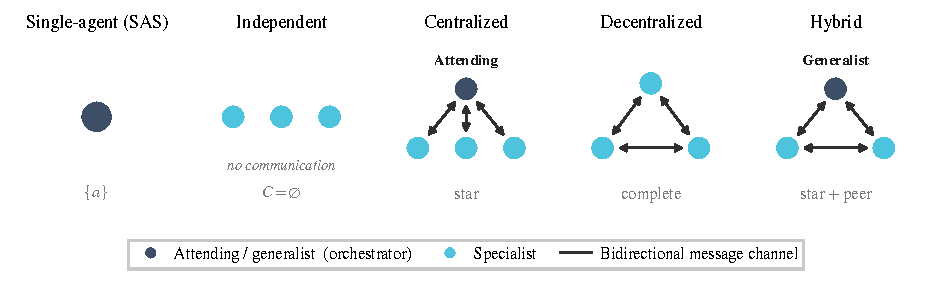
\includegraphics[width=\textwidth]{figures/fig0_architectures.pdf}
\caption{\textbf{The five architectures we evaluate}, with the clinical role each instantiates.
$A$ is the agent set, $C$ the communication graph, $\Omega$ the aggregation rule.}
\label{fig:arch}
\end{figure*}

\subsection{System definition}

We describe an agent system as a triple $(A, C, \Omega)$: a set of agents $A$, a communication graph $C$, and an aggregation rule
$\Omega$. Figure~\ref{fig:arch} and Table~\ref{tab:arch} give the five configurations we evaluate, each paired with the clinical role
it instantiates. The taxonomy is the one used for general-domain agent
systems~\citep{kim2026scaling}; the clinical instantiations are ours. Only the coordination logic differs across architectures. The item
rendering, the answer schema, the role prompts and the decoding parameters are shared.

\begin{table*}[t]\centering\small
\caption{Architectures, their coordination structure, and the clinical role each instantiates. $n$ is the panel size, $k$ reasoning iterations, $r$ orchestration rounds,
$d$ debate rounds.}
\label{tab:arch}
\begin{tabular}{@{}llll@{}}
\toprule
Architecture & $(A, C, \Omega)$ & Cost & Clinical instantiation \\
\midrule
Single-agent (SAS) & $\{a\}$ & $O(k)$ & One physician, zero-shot or CoT \\
Independent & $\{a_1..a_n\}$, $C=\emptyset$, synthesis & $O(nk)$ & Specialists answer blind; majority vote \\
Centralized & $+a_{\mathrm{orch}}$, star, hierarchical & $O(rnk)$ & \textbf{Attending physician} audits, then decides \\
Decentralized & $\{a_1..a_n\}$, complete, consensus & $O(dnk)$ & Multidisciplinary team discussion \\
Hybrid & $+a_{\mathrm{orch}}$, star + peer, both & $O(rnk{+}pn)$ & Tiered referral: triage $\rightarrow$ panel $\rightarrow$ MDT \\
\bottomrule
\end{tabular}
\end{table*}

\paragraph{Independent.} $N$ specialists receive the item and answer without seeing one another.
Aggregation is majority vote, ties broken by mean self-reported confidence and then by option
order. A confidence-weighted variant is logged throughout.

\paragraph{Centralized (attending physician).} An orchestrator receives the $N$ specialist
opinions on a star topology and is instructed to \emph{audit before aggregating}. It must name the
single opinion most likely to be wrong and justify that, then either commit to an answer or
re-task one named specialty. A re-tasked specialist re-answers with the orchestrator's critique in
hand. The star topology is preserved, since specialists never see each other. This design gives
the panel a single point at which errors can be caught before they reach the output, and it is the
architecture responsible for both the largest gain and the largest loss in the study.

\paragraph{Decentralized (MDT discussion).} $N$ specialists give first opinions, then exchange
opinions on a complete graph for up to three rounds, each free to revise. Rounds stop early only
on true unanimity, defined as every agent emitting the same \emph{valid} option. A panel
containing unparsed answers is not unanimous.

\paragraph{Hybrid (tiered referral).} A generalist answers first with a stated confidence. Below a
frozen threshold $\theta$ the case is referred to the $N$-specialist panel; if that panel has no
majority the case escalates to full MDT discussion. $\theta$ is calibrated once on a 100-item
development slice disjoint from every evaluation set and then frozen.

\paragraph{Panel composition.} A cheap router (\texttt{gpt-4.1-nano}, temperature 0) ranks the
nine most relevant specialties for each item from a fixed 17-specialty roster; a panel of size $N$
is the first $N$ of that ranking. Panels are therefore \emph{nested}: the $N{=}9$ panel contains
the $N{=}5$ panel, which contains the $N{=}3$ panel.

\subsection{Nested panels as common random numbers}
\label{sec:nested}

Every agent's first opinion is keyed on $(\text{item}, \text{specialty}_i, \text{seed}, i)$ and
never on $N$ or on the architecture. Consequently the first opinions of a panel of size $N$ are a
superset of those for any $N' < N$, and all four multi-agent architectures reuse the same first
opinions. This is a deliberate common-random-numbers coupling. It reduces the variance of
within-item contrasts between architectures and panel sizes, and it changes the estimand: we
measure \emph{accuracy as the same routed panel is extended}, not the expected accuracy of
independently redrawn panels at each size. Paired McNemar tests on item-level outcomes remain
valid under this coupling; regression models must cluster at the item level rather than treat
configurations as independent.

\subsection{What we measure}
\label{sec:metrics}

Accuracy alone cannot distinguish a panel that pools complementary evidence from one that repeats
itself, so we instrument each episode with five coordination quantities and one derived quantity
that the rest of the paper turns on.

We measure five coordination quantities. Their names are established in the agent-scaling
literature~\citep{kim2026scaling}, which reports headline values without always giving closed
forms; the definitions below are the ones we compute.

\begin{itemize}\itemsep2pt
\item \textbf{Turns} $T$: reasoning--response exchanges; one model call is one turn.
\item \textbf{Message density} $c$: peer-opinion exposures per turn. Independent has
$C = \emptyset$ and therefore $c = 0$ by construction; Centralized exposes opinions only to the
orchestrator; Decentralized and Hybrid expose every agent to every other each round.
\item \textbf{Redundancy} $R$: mean pairwise Jaccard overlap of rationale tokens among first
opinions. High $R$ means the panel is restating one another rather than contributing independent
information.
\item \textbf{Overhead} $O\%$: token cost relative to the single-agent baseline on the same items,
$(\mathrm{tok}_{\mathrm{MAS}} - \mathrm{tok}_{\mathrm{SAS}})/\mathrm{tok}_{\mathrm{SAS}}$.
\item \textbf{Coordination efficiency} $\Ec$: accuracy divided by the token-cost ratio to the
single-agent baseline.
\item \textbf{Error amplification} $\Ae$: the extent to which individual-agent errors reach the
final output without inter-agent verification. We measure that failure directly, in which the panel
\emph{held} the correct option among its first opinions and still emitted a wrong one,
normalised by the marginal probability that a single agent is wrong. $\Ae > 1$ means the system
destroys information it already possessed.
\end{itemize}

\paragraph{Effective independent opinions.}
Majority voting converts independent judgements into accuracy; correlated judgements it merely
repeats. We therefore summarise a panel not by its size but by how many independent opinions it
carries. Writing $\varphi$ for the mean pairwise error correlation between panel positions,
measured as the correlation of their per-item error indicators, the effective number of
independent opinions in a panel of $N$ agents is
\begin{equation}
N_{\mathrm{eff}} = \frac{N}{1 + (N-1)\varphi}.
\label{eq:neff}
\end{equation}
At $\varphi = 0$ the $N$ opinions are fully independent and $N_{\mathrm{eff}} = N$; at
$\varphi = 1$ they are one opinion copied $N$ times and $N_{\mathrm{eff}} = 1$. This is the
standard design-effect correction for clustered observations, and it makes the arithmetic premise
of consultation measurable rather than assumed. Reporting $N_{\mathrm{eff}}$ alongside $N$ turns
out to explain why panel size predicts so little (\S\ref{sec:premise}).

\subsection{Clinical tasks and benchmarks}

Three benchmarks, 250 items each, sampled with a fixed seed:
MedXpertQA-Text~\citep{zuo2025medxpertqa} (10 options; stratified by the 12 body systems $\times$
3 task types), MedQA-USMLE~\citep{jin2021medqa} (4 options), and the contamination-screened hard
split of MedAgentsBench~\citep{medagentsbench} (894 items excluding the
\texttt{medqa\_5options} subset; the first 250 after stratified shuffling). The primary endpoint
is exact match against the dataset's own gold option key. No LLM judge appears anywhere in the
evaluation path.

Every item is additionally tagged easy / medium / hard by the pass rate of three mid-tier models
at $k{=}5$ samples. On MedXpertQA the
strata are heavily skewed hard (13 / 62 / 125 on the pilot sample), which is the intended regime.

